\documentclass{article}
\usepackage{ctex}
\usepackage{fontspec}
\usepackage{listings}
\usepackage{xcolor}
\usepackage{geometry}
\usepackage{graphicx}
\usepackage{float}
\usepackage{amsmath}
\usepackage{minted}
\usepackage{tabularx}
\usepackage{makecell}
\usepackage{array}
\usepackage{booktabs}
\usepackage{algorithm2e}
\geometry{a4paper,scale=0.8}
\definecolor{codebg}{rgb}{0.95,0.95,0.95}
\begin{document}
\title{\Huge \centering \textbf{支持向量机($Support\ Vector \ Machine$)}}
\date{}
\maketitle
\setlength{\parskip}{0.5\baselineskip}
\section*{\LARGE 一、实验目的}

1. 理解支持向量机 ($SVM$) 的原理和应用。\\
\indent2. 掌握 $SVM$ 模型的训练和预测过程。\\
\indent3. 熟悉 $SVM$ 算法的参数设置和优化。

\section*{\LARGE 二、实验原理}
$SVM$,全称为支持向量机($Support\ Vector\ Machine$),是一种用于分类和回归分析的监督学习模型。在分类任务中,$SVM$试图将不同类别的数据集分隔开,并找到一个最优的超平面($hyperplane$)作为分类边界线($decision\ boundary$)。$SVM$的优点是可以处理高维数据集,且在解决小样本、非线性和高维模式识别时表现良好。

$SVM$的训练目标是找到一个最大间隔($Maximum\ Margin$)超平面,使得所有的数据点在最大间隔的两侧,即正类别和负类别。这个超平面可以定义为:
$$\mathbf{w}^T\mathbf{x}+b=0$$

其中$\mathbf{w}$为超平面的法向量,$b$为偏置($bias$)项。

为了最大化间隔,$SVM$需要寻找一组最优的参数$\mathbf{w}, b$,满足以下约束条件:
$$y_i(\mathbf{w}^T\mathbf{x_i}+b) \geq 1, i =1,...,n$$

其中$y_i$表示第$i$个数据点的类别($y_i=1$表示正类别,$y_i=-1$表示负类别),$n$表示数据点个数。

上述条件要求所有的数据点都被正确分类(即满足$y_i(\mathbf{w}^T\mathbf{x_i}+b)>0$),并且到最近的超平面距离(即间隔)必须大于等于1。在满足这些约束条件的基础上,$SVM$最大化间隔,即最小化$\lVert \mathbf{w} \rVert^2$,其中$\lVert \mathbf{w} \rVert$表示$\mathbf{w}$的欧几里得长度。

对于软间隔$SVM$,我们向其中加入松弛变量$\xi_i$,约束就变为
$$y_i(\mathbf{w}^T\mathbf{x_i}+b) \geq 1-\xi_i, i =1,...,n$$
它表示允许一些点以$\xi_i$的距离“侵入间隔”,当然这样做是需要支付一定代价的,我们会在目标函数中加入对应的惩罚项。

上述优化问题可以表示为以下约束优化问题:
$$\underset{\mathbf{w},b,\xi}{minimize} \cfrac{1}{2} \lVert \mathbf{w} \rVert^2+C\sum_{i=1}^{n}\xi_i$$
$$ subject\ to\ \  y_i(\mathbf{w}^T\mathbf{x_i}+b)\geq1-\xi_i, \xi_i>0,\ i =1,...,n$$

这是一个凸二次规划问题,可以采用拉格朗日乘子法(Lagrange Multiplier)求解。设$\alpha_i$为第$i$个数据点的拉格朗日乘子,$\beta_i$是对应每个样本的松弛变量$\xi_i$的乘子,对于任意的$i$,有:
$$L(\mathbf{w},b,\alpha,\xi,\mu)=\cfrac{1}{2} \lVert \mathbf{w} \rVert^2+C\sum_{i=1}^{n}\xi_i-\sum_{i=1}^{n} \left( \alpha_iy_i(\mathbf{w}^T\mathbf{x_i}+b)-\alpha_i+\alpha_i\xi_i\right)-\sum_{i=1}^{n}\mu_i\xi_i$$

其中$\alpha_i\geq 0,\ \mu_i\geq 0$,于是原问题可以用$Lagrange$函数来描述
$$\underset{\mathbf{w},b,\xi}{minimize}\ \underset{\alpha,\mu}{maximize}\ L(\mathbf{w},b,\alpha_i,\beta_i)$$

而原问题的$Lagrange$对偶问题写为:
$$\underset{\alpha,\mu}{maximize}\ \underset{\mathbf{w},b,\xi}{minimize}\ L(\mathbf{w},b,\alpha_i,\xi_i)$$

我们从对偶问题入手,先考虑里面的$\underset{\mathbf{w},b}{minimize}\ L(\mathbf{w},b,\alpha_i)$,我们首先对目标变量求导:
$$\cfrac{\partial L}{\partial \mathbf{w}}=0 \Rightarrow \mathbf{w}=\sum_{i=1}^n \alpha_iy_i\mathbf{x_i}$$
$$\cfrac{\partial L}{\partial b}=0 \Rightarrow \sum_{i=1}^n \alpha_iy_i=0$$
$$\cfrac{\partial L}{\partial \xi_i}=0 \Rightarrow C=\alpha_i+\mu_i$$

带回优化问题,得到:
$$\underset{\alpha}{minimize}\ -\sum_{i=1}^n \alpha_i+\cfrac{1}{2}\sum_{i=1}^    n \sum_{j=1}^n\alpha_i\alpha_jy_iy_j\mathbf{x_i}^T\mathbf{x_j}$$
$$ subject\ to\ \  C\geq \alpha_i \geq 0, \sum_{i=1}^n \alpha_iy_i=0$$

其中$\alpha$为拉格朗日乘子向量,而另一个乘子$\mu$被消去了,这时可以用凸二次规划算法求解。要指出的是,计算得到的$\alpha$必须要满足$KKT$条件,原始$KKT$条件包括以下四个方程式:

1. $Primal\ feasibility$:
$$y_i(w^T\phi(x_i)+b)-1 \ge 0$$
\indent2. $Dual\ feasibility$:
$$\alpha_i \ge 0$$
\indent3. $Complementary\ slackness$:
$$\alpha_i[y_i(w^Tx_i+b)-1] = 0$$
\indent4. $Karush-Kuhn-Tucker\ (KKT)$:
$$\nabla_wL(w,b) = 0$$

这些条件确保了$SVM$分类器可以找到全局最优解,并且在所有限制条件下实现最优化。
最终找到一组满足约束条件的$\alpha$后,就可以根据上述公式计算出具体的超平面。对于新的数据点$\mathbf{x}$,可以用以下公式判断其类别:
$$f(\mathbf{x})=sign(\sum_{i=1}^n \alpha_i y_i \mathbf{x_i}^T \mathbf{x}+b)$$

其中$sign$表示取符号函数。如果$f(\mathbf{x})>0$,则$\mathbf{x}$属于正类别;如果$f(\mathbf{x})<0$,则$\mathbf{x}$属于负类别。如果$f(\mathbf{x})=0$,则$\mathbf{x}$位于分类边界线上。

在实现$SVM$时,常用的方法是通过核函数$(Kernel\ Function)$将非线性问题转化为线性问题。核函数是一种将数据映射到高维空间的函数,可以将数据从低维空间线性可分转变为高维空间线性可分。常用的核函数有以下几种:

1. 线性核函数$(Linear\ Kernel\ Function)$:$K(\mathbf{x_i},\mathbf{x_j})=\mathbf{x_i}^T\mathbf{x_j}$,用于处理线性可分问题。

2. 多项式核函数$(Polynomial\ Kernel\ Function)$:$K(\mathbf{x_i},\mathbf{x_j})=(\gamma\mathbf{x_i}^T\mathbf{x_j}+r)^d$,其中$\gamma$、$r$和$d$是可调参数,用于处理多项式模型。

3. 高斯核函数$(Gaussian\ Kernel\ Function)$:$K(\mathbf{x_i},\mathbf{x_j})=\exp\{\cfrac{-\lVert \mathbf{x_i}- \mathbf{x_j} \rVert^2}{2\sigma^2}\}$,其中$\sigma$是可调参数,用于处理非线性模型。

4. Sigmoid核函数$(Sigmoid\ Kernel\ Function)$:$K(\mathbf{x_i},\mathbf{x_j})=\tanh(\gamma\mathbf{x_i}^T\mathbf{x_j}+r)$,其中$\gamma$和$r$是可调参数,用于处理sigmoid模型。

解决$SVM$问题的关键就是解决对应的凸优化问题,梯度下降$GD$理论上来说也可以解决$SVM$问题,但是实际中的使用非常少,这里我们主要介绍两种方法序列最小优化$SMO$算法和增广拉格朗日函数法$ALM$。

\subsection*{\Large 1、$SMO$算法}
SMO算法是一种二次规划的优化算法,其核心思想是将原问题分解为一系列子问题来求解,每个子问题只包含两个变量,通过对这两个变量进行优化来求解整个问题。将原本多变量规划问题转化为多次线性规划问题
逐步求解。

原问题为:
$$\max\limits_{\alpha}\sum_{i=1}^{N}\alpha_i-\cfrac{1}{2}\sum_{i=1}^{N}\sum_{j=1}^{N}y_iy_j\alpha_i\alpha_jK(x_i,x_j)$$
$$\begin{cases}
\sum\limits_{i=1}^N y_i\alpha_i=0 \\ 
0 \leq \alpha_i \leq C,i=1,2,\cdots,N \\
\end{cases}$$

其中,$\alpha$是拉格朗日乘子,$x_i$是样本点,$y_i$是标签,$K(x_i,x_j)$是核函数。

SMO算法的主要步骤如下:

1. 初始化拉格朗日乘子$\alpha$为0,选取两个不同的拉格朗日乘子$\alpha_i$和$\alpha_j$作为子问题;

2. 固定其他拉格朗日乘子,将子问题转化为一个只包含$\alpha_i$和$\alpha_j$的二次规划问题;

3. 求解二次规划问题,得到更新后的$\alpha_i$,$\alpha_j$以及$b$;

4. 重复以上步骤,直到满足终止条件。一般来说可以在尽可能多的样本点满足$KKT$条件后退出循环。

第一步选择的两个不同的拉格朗日乘子是非常关键的一步,一般来说我们采用两重循环(内循环和外循环)的方式来启发式选择更新的两个$\alpha$,假设选择的第一个乘子为$\alpha_i$,第二个为$\alpha_j$,
那么我们有如下选择策略:

在外循环中,首先进行全样本的遍历,选择一个不满足$KKT$条件的点对应的$\alpha$作为$\alpha_i$的选择。这时候可以进行内循环,继续选择第二个参数$\alpha_j$。第一次之后的外循环就转为使用边界样本点遍历,也就是
违反$0\leq\alpha\leq C\Leftrightarrow y_ig(x_i)=1$条件的点,从中选择一个作为$\alpha_i$。

在内循环中,我们的任务是选择一个$\alpha_j$,可以随机选择,也可以使用启发式选择。前者需要的迭代次数会更多,后者反之。为了介绍启发式选择的策略,我们首先引入预测误差。假设
$E_i$和$E_j$分别是样本$x_i$和$x_j$的预测误差,有:
$$E_i=f(x_i)-y_i=\sum_{k=1}^{N}\alpha_ky_kK(x_k,x_i)+b-y_i$$
$$E_j=f(x_j)-y_j=\sum_{k=1}^{N}\alpha_ky_kK(x_k,x_j)+b-y_j$$
在所有不满足$KKT$条件的非边界点中,我们优先选择使得$|E_i-E_j|$最大的点作为$\alpha_j$的选择,这样就保证了每次更新都有足够大的幅度,快速逼近收敛位置。

如果在某一轮迭代中,$\alpha$的更新非常小或者甚至没有更新,那么外循环重新改为全样本遍历。

SMO算法的核心在于如何求解子问题中的二次规划问题,在这里使用了坐标轮换算法,即固定所有$\alpha$,只对$\alpha_i$和$\alpha_j$进行更新。使用以下公式更新$\alpha_i$和$\alpha_j$:
$$\begin{cases}
\alpha_j^{new}=\alpha_j^{old}+\cfrac{y_j(E_i-E_j)}{\eta}\\
\alpha_i^{new}=\alpha_i^{old}+y_iy_j(\alpha_j^{old}-\alpha_j^{new}) \\
\end{cases}$$
其中,$\eta=K(x_i,x_i)+K(x_j,x_j)-2K(x_i,x_j)$,$K(\dot)$表示核函数,在线性支持向量机即为两个样本特征向量的内积。

而参数$b$的更新则按下列方式更新:首先根据$i$和$j$计算$b$的更新值:
$$b_i^{new}=-E_i-y_iK(x_i,x_i)(\alpha_i^{new}-\alpha_i^{old})-y_jK(x_i,x_j)(\alpha_j^{new}-\alpha_j^{old})+b^{old}$$
$$b_j^{new}=-E_j-y_jK(x_j,x_j)(\alpha_j^{new}-\alpha_j^{old})-y_iK(x_i,x_j)(\alpha_i^{new}-\alpha_i^{old})+b^{old}$$
理论上来说,这两个值都是合理的$b^{new}$,所以我们采用折中处理的方式令
$$b^{new}=\cfrac{b_i^{new}+b_j^{new}}{2}$$

更新后的$\alpha_i^{new}$和$\alpha_j^{new}$仍需要满足约束条件:
$$\begin{cases}
C\geq\alpha_i,\alpha_j\geq 0 \\
y_i\alpha_i^{new}+y_j\alpha_j^{new}=y_i\alpha_i+y_j\alpha_j \\
\end{cases}$$


最后,我们给出SMO算法的伪代码流程

\begin{algorithm}[H]
    \caption{SMO算法}
    \KwIn{训练数据集$D = \{(x_1,y_1),(x_2,y_2),\dots,(x_n,y_n)\}$,误差容忍度$\epsilon$,软间隔惩罚参数$C$}
    \KwOut{近似解$\alpha^{*}, b^{*}$}
    初始化 $\alpha_1= \alpha_2 = \dots = \alpha_n = b = 0$\\
    \While{iternum<max}{
        按照上述策略选择$\alpha_i$\\
        按照上述启发式策略选择另一个变量$\alpha_j$\\
        求解两个变量的二次规划问题以更新$\alpha_1$,$\alpha_2$以及$b$\\
        如果$\alpha_i$和$\alpha_j$都满足$KKT$条件或者$\alpha_i$或$\alpha_j$不可再优,则继续选择处理$\alpha_i$的第一个变量进行优化\\
    }
    \Return $\alpha^{*} = (\alpha_1^{*},\alpha_2^{*},\dots,\alpha_n^{*}), b^{*}$
\end{algorithm} 
    

通过SMO算法,可以较快地求解$SVM$问题,并且可以处理大型数据集。由于只需要维护两个变量,因此SMO算法的空间复杂度也比较低。

\subsection*{\Large 2、$ALM$算法}
$ALM$算法的本质和梯度下降非常相似,但是不同的是$ALM$算法在计算拉格朗日函数的过程中加入了一项增广项用于解决目标函数光滑性的问题。
我们首先给出目标函数的优化问题
$$\underset{\alpha}{minimize}\ -\sum_{i=1}^n \alpha_i+\cfrac{1}{2}\sum_{i=1}^    n \sum_{j=1}^n\alpha_i\alpha_jy_iy_j\mathbf{x_i}^T\mathbf{x_j}$$
$$ subject\ to\ \  C\geq \alpha_i \geq 0, \sum_{i=1}^n \alpha_iy_i=0$$

为了得到$\alpha$的取值,我们构建增广拉格朗日函数
$$L(\alpha,\lambda;\beta)=-\sum_{i=1}^n \alpha_i+\cfrac{1}{2}\sum_{i=1}^{n} \sum_{j=1}^n\alpha_i\alpha_jy_iy_j\mathbf{x_i}^T\mathbf{x_j}+\sum_{i=1}^{n}\lambda\alpha_iy_i+\cfrac{\beta}{2}\sum_{i=1}^{n}(y_i\alpha_i)^2$$
其中的$\cfrac{\beta}{2}\sum_{i=1}^{n}(y_i\alpha_i)^2$是罚函数项,而$\sum_{i=1}^{n}\lambda\alpha_iy_i$是拉格朗日乘子项。
为了便于后续的书写,我们将其中的向量用矩阵来替换,拉格朗日函数重写为:
$$L(\alpha,\lambda;\beta)=\cfrac{1}{2}\alpha^T(\hat{Y}\circ X)(\hat{Y}\circ X)^T\alpha-1^T\alpha+\lambda Y^T\alpha+\cfrac{\beta}{2}(Y^T\alpha)$$
其中$X=\begin{bmatrix}\mathbf{x}_1^T\\\mathbf{x}_2^T\\\vdots\\\mathbf{x}_n^T\end{bmatrix}$,
$Y=\begin{bmatrix}y_1\\y_2\\\vdots \\y_n\end{bmatrix}$,
而$\hat{Y}=\begin{bmatrix}\mathbf{y}_1^T\\\mathbf{y}_2^T\\\vdots\\\mathbf{y}_n^T\end{bmatrix}$,
$\mathbf{y}_i^T=[y_i,y_i\dots,y_i]$,$\mathbf{y}_i$的维数等于$\mathbf{x}_i$的维数。

按照梯度下降的思想,我们给出$ALM$中参数更新的公式
$$\hat{\alpha}^k=\alpha^k-\eta\nabla L(\alpha^k,\lambda^k)=\alpha^k-\eta((\hat{Y}\circ X)(\hat{Y}\circ X)^T\alpha^k-1+\lambda^kY+\beta Y^T\alpha^kY)$$
由优化问题中的约束,对$\hat{\alpha^k}$剪枝得到
$$\alpha_i^{k+1}=\begin{cases}\alpha_i^k,\ \ 0\leq\hat{\alpha}_i^k\leq C\\
0,\ \ \hat{\alpha}_i^k<0\\
C, \ \ \hat{\alpha}_i^k>C \end{cases}$$
$\lambda$的更新在$\alpha$更新之后完成
$$\lambda^{k+1}=\lambda^k+\beta(Y^T\alpha^{k+1})$$
最后我们同样给出伪代码流程

\begin{algorithm}[H]
    \caption{ALM算法}
    \KwIn{训练数据集$D = \{(x_1,y_1),(x_2,y_2),\dots,(x_n,y_n)\}$,误差容忍度$\epsilon$,软间隔惩罚参数$C$}
    \KwOut{近似解$\alpha^{*}, b^{*}$}
    初始化 $\alpha_1= \alpha_2 = \dots = \alpha_n = b = 0$,$\lambda=0$,$\eta=\cfrac{0.03}{n}$\\
    \While{iternum<max}{
        计算$\hat{\alpha}^k=\alpha^k-\eta\nabla L(\alpha^k,\lambda^k)=\alpha^k-\eta((\hat{Y}\circ X)(\hat{Y}\circ X)^T\alpha^k-1+\lambda^kY+\beta Y^T\alpha^kY)$\\
        对$\hat{\alpha}^k$剪枝得到更新后的$\alpha^{k+1}$\\
        计算$\lambda^k+\beta(Y^T\alpha^{k+1})$更新$\lambda$\\
        \If{all satisfy kkt or update too small}{break}
    }
    \Return $\alpha^{*} = (\alpha_1^{*},\alpha_2^{*},\dots,\alpha_n^{*}), b^{*}$
\end{algorithm} 
\section*{\LARGE 三、实验步骤}
\indent1、生成不同中心的正态随机样本点,包括线性可分和线性不可分的样本。\\
\indent2、完成$ALM$和$SMO$算法实现的$SVM$。\\
\indent3、验证$SVM$,并尝试调整参数,观察现象。

\section*{\LARGE 四、实验代码}
\noindent 样本的生成以及超平面可视化
\begin{minted}[linenos,breaklines,bgcolor=codebg]{python3}
import numpy as np
import matplotlib.pyplot as plt

np.random.seed(25565)
center1=np.array([1,1])
center2=np.array([3,3])
sample1=np.random.randn(200,2)
sample2=np.random.randn(200,2)
sample1=sample1+center1
sample2=sample2+center2
tag1=np.ones(200)
tag2=np.ones(200)*(-1)

plt.scatter(sample1[:,0],sample1[:,1],marker='3',s=20)
plt.scatter(sample2[:,0],sample2[:,1],marker='3',s=20)

def print_line(omega:np.ndarray,b:float,line_style:str='solid'):
    x=np.linspace(-2,8)
    y=(-b-omega[0]*x)/omega[1]
    plt.plot(x,y,linestyle=line_style)
\end{minted}

\noindent $SVM$分类器的实现。由于这部分代码比较长,所以我们将其分开展示。首先是参数和相关可视化函数
\begin{minted}[linenos,breaklines,bgcolor=codebg]{python3}
class svm_classifier:
    def __init__(self, C=1.0, kernel='linear', max_iter=1000):
        self.C = C
        self.kernel = kernel
        self.max_iter = max_iter
        self.b=0
        self.epsilon=1e-3

        self._lambda=0
        self.beta=0.01
        self.eta=1e-4

    def kernel_function(self, x1:np.ndarray, x2:np.ndarray):
        if self.kernel == 'linear':
            return np.dot(x1, x2)
        elif self.kernel == 'gaussian':
            sigma = 1.0
            return np.exp(-np.linalg.norm(x1 - x2) ** 2 / (2 * (sigma ** 2)))

    def alpha2omega(self,alpha:np.ndarray,x:np.ndarray,y:np.ndarray)->np.ndarray:#convert alpha to omega
        omega=np.zeros(len(x[0]))
        for i in range(0,len(x)):
            omega+=alpha[i]*y[i]*x[i]
        return omega

    def mark_sv(self,x:np.ndarray,y:np.ndarray):# highlight the support vector and margin
        for idx,alpha in enumerate(self.alpha):
            if 0<alpha<self.C:
                plt.scatter(x[idx][0], x[idx][1], s=50, c='none', marker='o', edgecolors='blue')
        print_line(self.omega,self.b-1,'dashdot')
        print_line(self.omega,self.b+1,'dashdot')
\end{minted}

$SMO$算法所用到的代码
\begin{minted}[linenos,breaklines,bgcolor=codebg]{python3}
class svm_classifier:
    ...
    def refresh_E(self,x:np.ndarray,y:np.ndarray):
        Gx:np.ndarray=(self.alpha*y)*np.sum(x@x.T,axis=0)+self.b
        self.E:np.ndarray=Gx-y

    def selectJ(self,i:int,x:np.ndarray,y:np.ndarray,length:int): #call this function to obtain a j
        j:int=np.random.randint(0,length)
        while i==j:
            j=np.random.randint(0,length)

        random_factor=np.random.randint(0,100)
        maxK = -1
        maxDeltaE = 0
        idx=np.nonzero(self.alpha)[0]
        if(len(idx)!=0):
            for index in idx:
                if index==i:continue
                Eindex=self.g(x,index,y)-y[index]
                Ei=self.g(x,i,y)-y[i]
                # eta = self.kernel_function(x[i], x[i]) + self.kernel_function(x[index], x[index]) - 2 * self.kernel_function(x[i], x[index])
                eta=1
                deltaE=abs(Ei-Eindex)/eta
                if (deltaE > maxDeltaE):
                    maxK = index
                    maxDeltaE = deltaE
            # print('choose '+str(maxK))
            print(random_factor)
            if random_factor%7==0:
                print('random choice')
                return j
            else:
                return maxK
        return j

    def update_b(self,i:int,j:int,x:np.ndarray,y:np.ndarray):
        res1:float=y[i]
        res2:float=y[j]
        #if  and
        for k in range(0,len(x)):
            res1-=self.alpha[k]*y[k]*self.kernel_function(x[k],x[i])
            res2-=self.alpha[k]*y[k]*self.kernel_function(x[k],x[j])

        if -self.epsilon < self.alpha[i] < self.C+self.epsilon:
            self.b=res1
        elif -self.epsilon < self.alpha[j] < self.C+self.epsilon:
            self.b=res2
        else:
            self.b=(res1+res2)/2

    def g(self,x:np.ndarray,i:int,y:np.ndarray): #use to calculate the model output based on current alpha
        res:float=0
        index=[index for index,value in enumerate(self.alpha) if value != 0]
        for k in index:
            res+=self.alpha[k]*y[k]*self.kernel_function(x[i],x[k])
        return res+self.b

    def update(self,x:np.ndarray,y:np.ndarray,i:int,j:int=-1): #SMO update parameters
        alpha_update:bool=False
        if j==-1:
            j = self.selectJ(i, x,y,len(x))
        eta = self.kernel_function(x[i], x[i]) + self.kernel_function(x[j], x[j]) - 2 * self.kernel_function(x[i], x[j])
        if eta == 0: return -2

        self.E[i] = self.g(x, i, y) - y[i]
        self.E[j] = self.g(x, j, y) - y[j]

        if y[i]!=y[j]:
            L = max(0, self.alpha[j] - self.alpha[i])
            H = min(self.C, self.C + self.alpha[j] - self.alpha[i])
        else:
            L = max(0, self.alpha[j] + self.alpha[i] - self.C)
            H = min(self.C, self.alpha[j] + self.alpha[i])
        alpha_newj = \
            self.alpha[j] + (1) * y[j] * (self.E[i] - self.E[j]) / eta
        alpha_oldj = self.alpha[j]

        if alpha_newj > H:
            self.alpha[j] = H
        elif alpha_newj < L:
            self.alpha[j] = L
        else:
            self.alpha[j] = alpha_newj

        self.alpha[i] = self.alpha[i] + y[i] * y[j] * (alpha_oldj - self.alpha[j])
        self.update_b(i, j, x, y)

        self.E[i]=self.g(x,i,y)-y[i]
        self.E[j]=self.g(x, j, y) - y[j]
        if np.sum(np.abs(alpha_newj - self.alpha[j])) < 1e-10:
            return -2#-2 means tiny update, time to change a new strategy
        return 1#normal status

    def check_kkt(self,x:np.ndarray,i:int,y:np.ndarray)->bool: #check if a point is satisfied with kkt conditions
        kkt=False
        check_kkt=y[i]*self.g(x,i,y)
        if check_kkt>1-self.epsilon and -self.epsilon < self.alpha[i] < self.epsilon or \
                1-self.epsilon < check_kkt < 1+self.epsilon and -self.epsilon < self.alpha[
            i] < self.C + self.epsilon or \
                check_kkt<1+self.epsilon and self.C - self.epsilon < self.alpha[i] < self.C + self.epsilon:
            kkt=True
        return kkt

    def all_check_kkt(self,x:np.ndarray,y:np.ndarray)->bool: #check if all point is satisfied with kkt conditions. 
        kkt=False
        Gx:np.ndarray=self.alpha*y@(x@x.T)+self.b
        check_kkt:np.ndarray=y*Gx-1
        kkt_unsatisfy1=[idx for idx,value in enumerate(self.alpha) if check_kkt[idx]>-self.epsilon and (-self.epsilon>value or value>self.epsilon)]
        kkt_unsatisfy2=[idx for idx,value in enumerate(self.alpha) if self.epsilon>check_kkt[idx]>-self.epsilon and (value<self.epsilon or value>self.C-self.epsilon)]
        kkt_unsatisfy3=[idx for idx,value in enumerate(self.alpha) if check_kkt[idx]<self.epsilon and (self.C-self.epsilon<value or value<self.C+self.epsilon)]
        if len(kkt_unsatisfy1)==0 and len(kkt_unsatisfy2)==0 and len(kkt_unsatisfy3)==0:
            return True
        else: return False

    def train(self,x:np.ndarray,y:np.ndarray,max_internum:int): #SMO training
        self.alpha=np.zeros(len(x))
        self.omega=self.alpha2omega(self.alpha,x,y)
        self.E=np.zeros(len(x))
        iternum:int=0
        alpha_update: bool = False
        while(iternum<max_internum):
            if (not alpha_update) or iternum==1:
                alpha_update=True
                for i1 in range(0,len(x)):
                    if not self.check_kkt(x,i1,y):
                        self.update(x,y,i1)
            if alpha_update:
                alpha_update=False
                for i2 in range(0,len(x)):
                    if (self.epsilon>self.alpha[i2]>-self.epsilon and y[i2]*self.g(x,i2,y)<1+self.epsilon):
                        status:int=self.update(x,y,i2)
                        if status==1:
                            alpha_update=True
                    elif (self.C+self.epsilon>self.alpha[i2]>self.C-self.epsilon and y[i2]*self.g(x,i2,y)>1-self.epsilon):
                        status:int=self.update(x,y,i2)
                        if status==1:
                            alpha_update=True
            iternum+=1
            print(iternum)
            self.omega: np.ndarray = self.alpha2omega(self.alpha, x, y)
        self.mark_sv(x,y)
\end{minted}

\noindent 最后是$ALM$部分的代码
\begin{minted}[linenos,breaklines,bgcolor=codebg]{python3}
class svm_classifier:
    ...
    def _train_lagrange(self,x:np.ndarray,y:np.ndarray,iternum:int):
        iter=0
        yi=0.03
        x1=np.array([value*y[idx] for idx,value in enumerate(x)])
        self.alpha=np.zeros(len(x))
        while iter<iternum:
            alpha_old=self.alpha
            alpha_new=self.alpha-yi/len(x)*(x1@x1.T@self.alpha-1 + self._lambda*y+self.beta*y@self.alpha*y)
            alpha_new=np.where(alpha_new>self.C,self.C,alpha_new)
            alpha_new=np.where(alpha_new<0,0,alpha_new)
            self.alpha=alpha_new
            _lambda_old=self._lambda
            self._lambda=_lambda_old+self.beta/len(x)*(y@self.alpha)
            iter+=1
            if np.sum(abs(alpha_old-self.alpha))<1e-6:
                break
            print(np.sum(abs(alpha_old-self.alpha)))

        self.omega=self.alpha2omega(self.alpha,x,y)
        a1=np.array([value for idx,value in enumerate(self.alpha) if self.C>value>0])
        a2=np.array([value for idx,value in enumerate(a1) if np.max(a1)-0.01>value>np.min(a1)+0.01])
        op=np.median(a2)
        op1=np.min(abs(a2-op))
        j=np.argmin(abs(a2-op))
        op=a2[j]
        j=np.argmin(abs(self.alpha-op))
        u=0
        for _ in range(len(x)):
            u+=self.alpha[_]*y[_]*(x[_]@x[j])
        self.b=y[j]-u
        self.mark_sv(x,y)
        print_line(self.omega,self.b)
\end{minted}

\section*{\LARGE 五、实验结果}
上文所介绍的$SMO$算法和$ALM$算法都可以得到正确的答案,以下实验结果简单起见,统一采用$ALM$方法计算。

$SVM$的$C=1.0$,$\epsilon=1e-5$,$ALM$的参数$\beta=0.01$。当中心为$(1,1)$和$(6,6)$时,各样本点数量为$100$时,正负样本线性可分:
\begin{figure}[H]
    \centering
    \begin{minipage}[t]{1.0\linewidth}
        \centering
        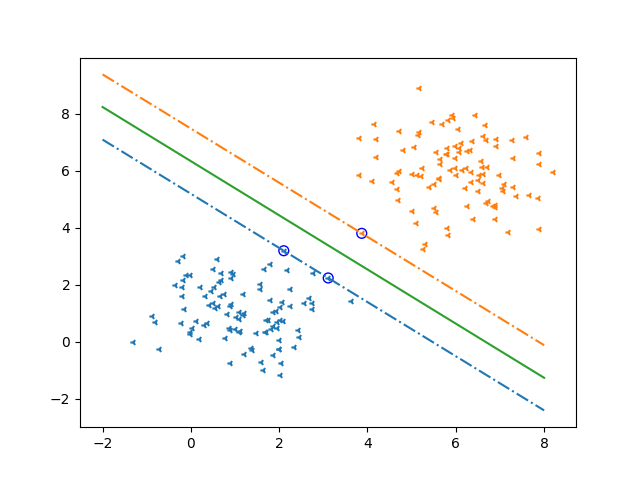
\includegraphics[height=8cm]{Figure_1.png}
        \caption{中心为$(1,1)$和$(6,6)$}
    \end{minipage}
 \end{figure}
 虚线表示的是$SVM$的间隔,蓝色圆圈所圈的点即为$SVM$的支持向量,整个$SVM$的超平面计算只与支持向量有关。

 调整样本中心为$(1,1)$和$(3,3)$,得到的实验结果
 \begin{figure}[H]
    \centering
    \begin{minipage}[t]{1.0\linewidth}
        \centering
        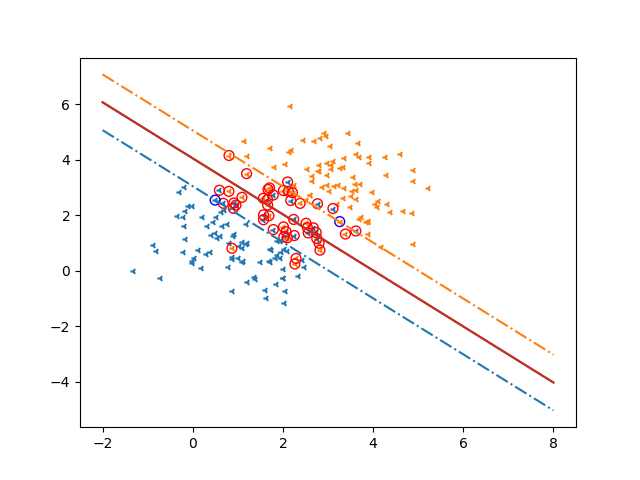
\includegraphics[height=8cm]{Figure_2.png}
        \caption{中心为$(1,1)$和$(4,4)$}
    \end{minipage}
 \end{figure}
 可以看到对于线性不可分的数据,$SVM$依然能够实现将大部分的样本完美分开,容忍部分样本点进入间隔内。

 \subsection*{\Large 附加题1: \textbf{参考《统计学习方法》-李航,解释间隔最大化或软间隔最大化,如何建模成$SVM$模型?如何由模型(1)得到对偶问题(2)?在线性可分和线性不可分问题中,如何定义支持向量?
}}
关于第一问的$SVM$模型的建立,可以参见实验原理部分。从基本的$SVM$模型到其对偶问题的推导,涉及到凸优化的理论,也就是拉格朗日对偶性的推导。为了简单期间,我们首先假设
原问题为:
\begin{align}
min\quad f_0(x)\\ s.t.\quad f_i(x)\preceq 0,\quad i=1,2\hdots ,m\\ h_i(x)=0,\quad i=1,2,\hdots,n
\end{align}

首先我们不妨考虑优化这么一个函数
$$min \ \mathcal{L}=f_0(x)+\sum_{i=1}^{m}I_{-}(f_i(x))+\sum_{i=1}^pI_0(h_i(x))$$
这里的$I_-$和$I_0$都是指示函数。即$I_{-}(u)=\left\{ \begin{aligned}0\quad u\leq0\\\infty\quad u>0\end{aligned}\right.$,$I_{0}(u)=\left\{ \begin{aligned}0\quad u=0\\\infty\quad u\ne0\end{aligned}\right.$
原来的线性约束条件通过指示函数的“惩罚”重新体现出来,也就是说,原来的$f_i(x)$只要大于$0$或者原来的$h_i(x)$只要不为$0$,都会引起$\mathcal{L}$函数值趋于正无穷而无法实现优化目标。我们记这个问题的解为$p\star$,这个解与原问题的解是等同的。

现在我们给出其拉格朗日函数形式
$$min\ L(x,\lambda,\nu) =f_0(x)+\sum_{i=1}^{m}\lambda_i f_i(x)+\sum_{i=1}^p\nu_ih_i(x)$$

结合上面的思想,换一个角度取理解这个拉格朗日函数,$f_0(x)$就是原函数的部分,而$\sum_{i=1}^{m}\lambda_i f_i(x)+\sum_{i=1}^p\nu_ih_i(x)$表示的是惩罚部分,也就是说,如果
存在某一个点违背了我们的约束条件,那么都会导致拉格朗日函数值的上升,但不至于趋于正无穷。我们记这问题的解为$g(\lambda,\nu)=\inf_{x\in D}\ L(x,\lambda,\nu)$,很显然有$g(\lambda,\nu)\leq p\star$。

这时可以考虑$\lambda$和$\nu$,我们希望获得最大的下界$g(\lambda,\nu)$,因为这样子我们的拉格朗日函数的解就是$p\star$,这就引出来我们的拉格朗日对偶问题:
\begin{align}max\quad g(\lambda,\nu)\\s.t.\quad \lambda\succeq 0\end{align}设对偶问题的解为$d\star$,由于下界函数$g(\lambda,\nu)$始终小于$p\star$,显然又有$d\star\leq p\star$成立,如果$d\star=p\star$成立,则原问题称为
强对偶。可以证明,当原问题满足$Slater$条件时,这个问题是强对偶问题,这是我们使用拉格朗日对偶问题求解$SVM$的原问题的基础。

在实验原理部分,我们已经指出原问题是如何转化为其拉格朗日对偶问题的。首先给出原问题
$$\underset{\mathbf{w},b,\xi}{minimize} \ \cfrac{1}{2} \lVert \mathbf{w} \rVert^2+C\sum_{i=1}^{n}\xi_i$$
$$ subject\ to\ \  y_i(\mathbf{w}^T\mathbf{x_i}+b)\geq1-\xi_i, \xi_i>0,\ i =1,...,n$$
变换为对应的拉格朗日函数得到
$$L(\mathbf{w},b,\alpha,\xi,\mu)=\cfrac{1}{2} \lVert \mathbf{w} \rVert^2+C\sum_{i=1}^{n}\xi_i-\sum_{i=1}^{n} \left( \alpha_iy_i(\mathbf{w}^T\mathbf{x_i}+b)-\alpha_i+\alpha_i\xi_i\right)-\sum_{i=1}^{n}\mu_i\xi_i$$
对应的问题写为
$$\underset{\mathbf{w},b,\xi}{minimize}\ L(\mathbf{w},b,\alpha_i,\beta_i)$$
但是这个问题的解与原问题的解可能并不一样,根据我们刚刚介绍的对偶性证明,我们希望将拉格朗日函数形式下的问题最大化,因为这样可以得到对应原问题的解$p\star$,于是对偶问题就是
$$\underset{\alpha,\mu}{maximize}\ \underset{\mathbf{w},b,\xi}{minimize}\  L(\mathbf{w},b,\alpha_i,\beta_i)$$

通过对目标变量求导,令其值为$0$,最终就可以得到:
$$\underset{\alpha}{maximize}\ \sum_{i=1}^n \alpha_i-\cfrac{1}{2}\sum_{i=1}^n \sum_{j=1}^n\alpha_i\alpha_jy_iy_j\mathbf{x_i}^T\mathbf{x_j}$$
$$ subject\ to\ \  C\geq \alpha_i \geq 0, \sum_{i=1}^n \alpha_iy_i=0$$
这在实验原理部分已经详尽介绍,注意这里的正负号取反,优化目标也取了反。

关于第三问的的支持向量,从定义上来说线性可分的SVM问题中,支持向量是指距离超平面最近的样本点,且这些样本点满足KKT条件中的支持向量条件。

在线性不可分的SVM问题中,支持向量是指在软间隔或者硬间隔条件下,约束条件最紧的样本点,即它们的拉格朗日乘子大于0。

数学角度上,对于线性可分的SVM问题,假设超平面为$w^Tx+b=0$,则支持向量可以表示为:

$$\begin{aligned} w^Tx_i+b&=1 \ \text{or} \ -1 \\ y_i(w^Tx_i+b)&\geq 1 \ \text{and} \ \alpha_i>0 \end{aligned}$$

其中,$y_i$为样本的标签,$\alpha_i$为对应样本的拉格朗日乘子,满足$\sum\limits_{i=1}^{m}\alpha_iy_i=0$。

对于线性不可分的SVM问题,假设超平面为$w^Tx+b=0$,则支持向量可以表示为:

$$\begin{aligned} y_i(w^Tx_i+b)& \geq 1-\xi_i \\ \alpha_i&>0 \end{aligned}$$

其中,$y_i$为样本的标签,$\alpha_i$为对应样本的拉格朗日乘子,$\xi_i$为样本的松弛变量,满足$0\leq \xi_i \leq C$。

\subsection*{\Large 附加题2: \textbf{学习增广拉格朗日法$(Augmented\ Lagrangian\ method)$,做笔记,调整参数$\beta$和步长,观察其对收敛速度的影响。
}}
笔记参见实验原理部分,其中$ALM$部分有详尽的算法介绍。在$ALM$中,$\beta$和$\eta$是$\lambda$以及$\alpha$更新必须的参数。
实验代码中,$ALM$退出迭代的标准是$\alpha$的变化的$L1$范数值小于$1e-6$退出,以默认的参数运行
\begin{minted}[linenos,breaklines,bgcolor=codebg]{python3}
model eta: 0.00015
model beta: 0.01
time consume: 19.271769523620605s
\end{minted}
运行结果图
\begin{figure}[H]
    \centering
    \begin{minipage}[t]{1.0\linewidth}
        \centering
        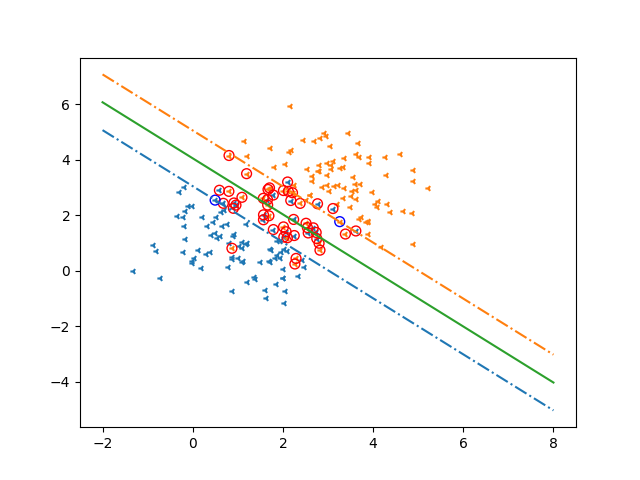
\includegraphics[height=8cm]{runtime_1.png}
        \caption{中心为$(1,1)$和$(3,3)$}
    \end{minipage}
 \end{figure}
 增大令$\eta=0.0003$
 \begin{minted}[linenos,breaklines,bgcolor=codebg]{python3}
    model eta: 0.0003
    model beta: 0.01
    time consume: 15.637076616287231s
    \end{minted}
\begin{figure}[H]
        \centering
        \begin{minipage}[t]{1.0\linewidth}
            \centering
            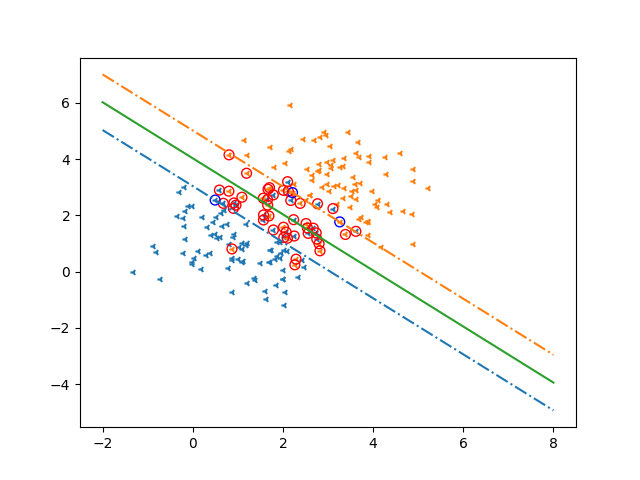
\includegraphics[height=8cm]{runtime_2.png}
            \caption{中心为$(1,1)$和$(3,3)$}
        \end{minipage}
     \end{figure}
     
继续增大令$\eta=0.0005$
\begin{minted}[linenos,breaklines,bgcolor=codebg]{python3}
    model eta: 0.0005
    model beta: 0.01
    time consume: 12.698193311691284s
    \end{minted}
\begin{figure}[H]
        \centering
        \begin{minipage}[t]{1.0\linewidth}
            \centering
            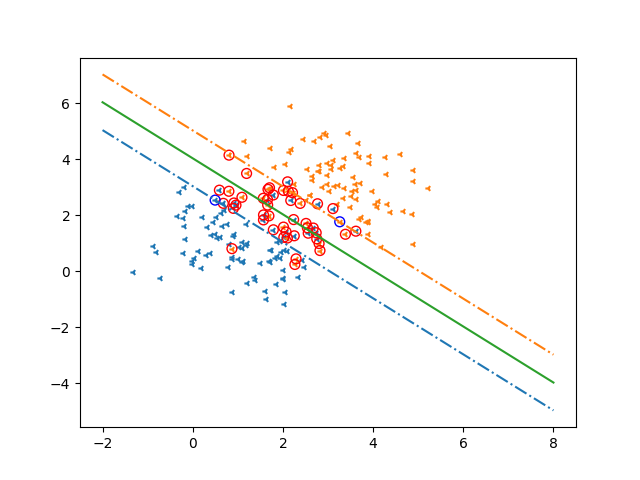
\includegraphics[height=8cm]{runtime_3.png}
            \caption{中心为$(1,1)$和$(3,3)$}
        \end{minipage}
     \end{figure}
不难看出,随着$\eta$的增大,收敛速度逐渐变快,但是如果$\eta$过大,会导致步长过长,参数的值会非常大,并且振荡非常激烈无法收敛,甚至出现$nan$的计算值。

尝试修改$\beta$值,令$\beta=0.03$
\begin{minted}[linenos,breaklines,bgcolor=codebg]{python3}
    model eta: 0.00015
    model beta: 0.03
    time consume: 19.3364896774292s
    \end{minted}
\begin{figure}[H]
        \centering
        \begin{minipage}[t]{1.0\linewidth}
            \centering
            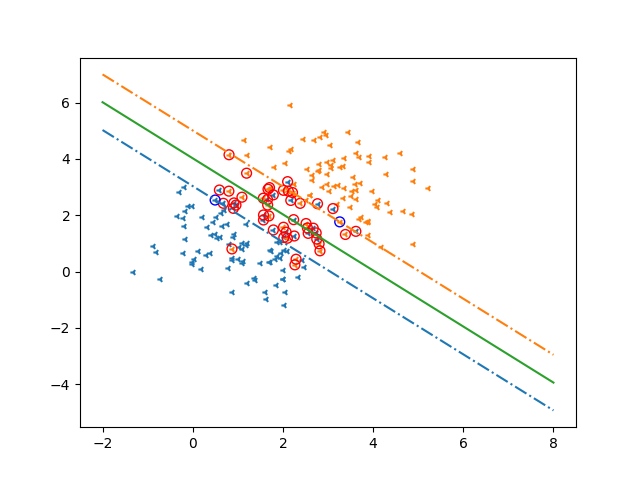
\includegraphics[height=8cm]{runtime_4.png}
            \caption{中心为$(1,1)$和$(3,3)$}
\end{minipage}
\end{figure}
相比于默认参数并没有加快,尝试继续增加令$\beta=0.09$
\begin{minted}[linenos,breaklines,bgcolor=codebg]{python3}
    model eta: 0.00015
    model beta: 0.09
    time consume: 21.18831706047058s
    \end{minted}
\begin{figure}[H]
        \centering
        \begin{minipage}[t]{1.0\linewidth}
            \centering
            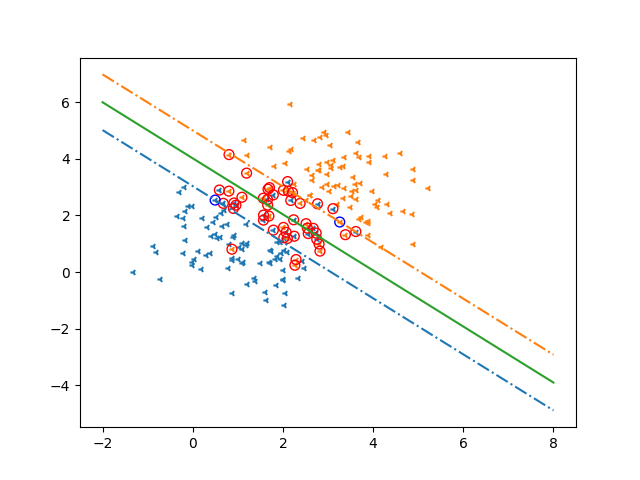
\includegraphics[height=8cm]{runtime_5.png}
            \caption{中心为$(1,1)$和$(3,3)$}
\end{minipage}
\end{figure}
收敛速度稍许增加,推测可能是由于步长过长导致振荡次数增加。尝试减小为$\beta=0.012$
\begin{minted}[linenos,breaklines,bgcolor=codebg]{python3}
    model eta: 0.00015
    model beta: 0.012
    time consume: 18.74616813659668s
    \end{minted}
\begin{figure}[H]
        \centering
        \begin{minipage}[t]{1.0\linewidth}
            \centering
            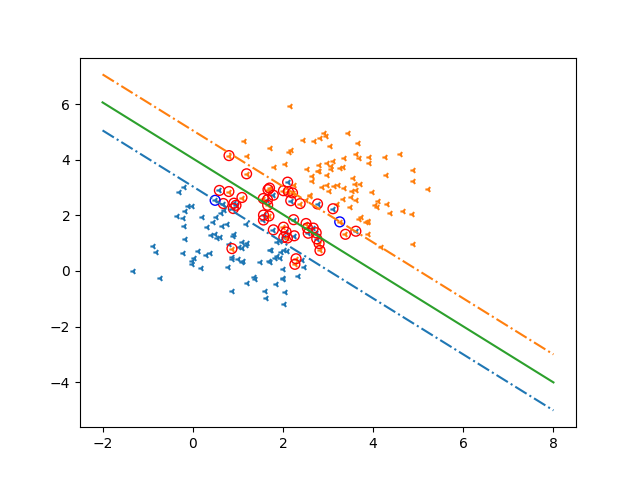
\includegraphics[height=8cm]{runtime_6.png}
            \caption{中心为$(1,1)$和$(3,3)$}
\end{minipage}
\end{figure}
运算速度稍有提升,基本可以确定$0.01$左右的值是较优值。

\subsection*{\Large 附加题3: \textbf{调参数$C$,观测其对分类效果的影响
}}
参数$C$影响模型对进入间隔的容忍程度。为了能够显示这一特性,我们选择一个基本可以线性可分的情况。
令两个样本中心分别为$(1,1)$和$(5,5)$,当$C=1.0$时
\begin{figure}[H]
    \centering
    \begin{minipage}[t]{1.0\linewidth}
        \centering
        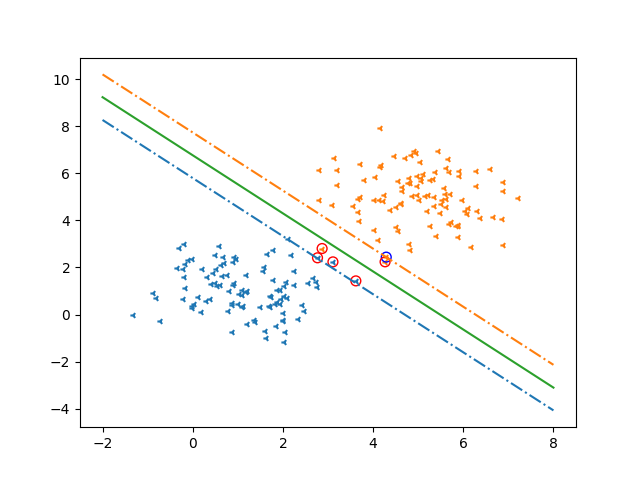
\includegraphics[height=8cm]{1c.png}
        \caption{中心为$(1,1)$和$(5,5)$,$C=1.0$}
\end{minipage}
\end{figure}
可以看到模型的支持向量有$6$个,现在调整$C=10.0$
\begin{figure}[H]
    \centering
    \begin{minipage}[t]{1.0\linewidth}
        \centering
        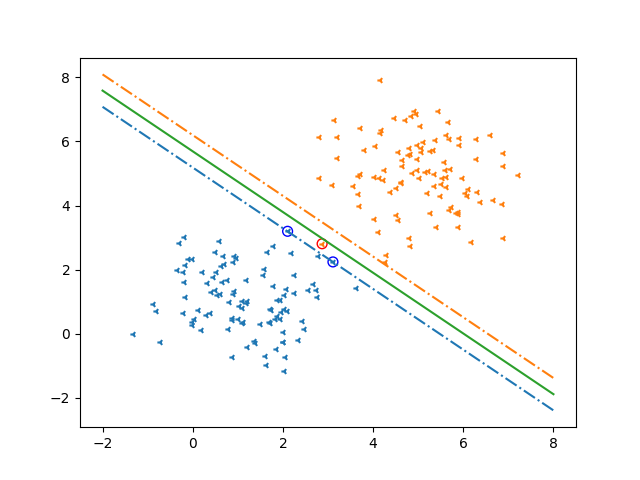
\includegraphics[height=8cm]{10c.png}
        \caption{中心为$(1,1)$和$(5,5)$,$C=10.0$}
\end{minipage}
\end{figure}
由于$C$的增大,模型对松弛点的容忍度降低,模型重新调整了$\omega$,使得函数间隔减小,间隔内的支持向量减少为$3$个。
尝试继续增大令$C=100.0$
\begin{figure}[H]
    \centering
    \begin{minipage}[t]{1.0\linewidth}
        \centering
        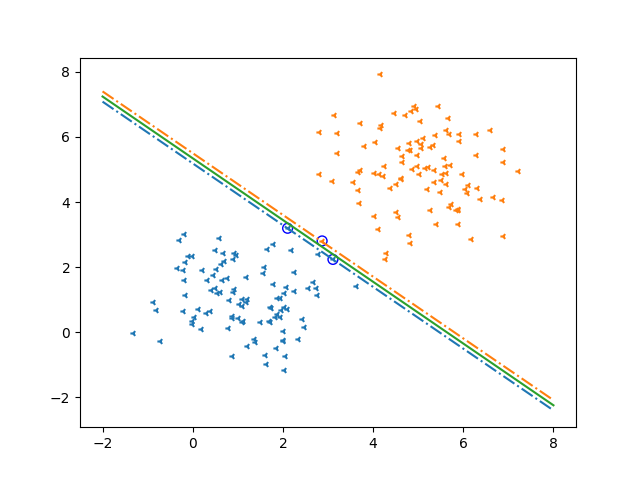
\includegraphics[height=8cm]{100c.png}
        \caption{中心为$(1,1)$和$(5,5)$,$C=100.0$}
\end{minipage}
\end{figure}
调整之后仍然是三个支持向量,但三个支持向量都是边界支持向量,这说明模型目前几乎不能容忍任何松弛点进入间隔。
\end{document}